\documentclass[conference]{IEEEtran}
\usepackage{cite}
\usepackage{amsmath,amssymb,amsfonts}
\usepackage{graphicx}
\usepackage{textcomp}
\usepackage{xcolor}
\usepackage{booktabs}
\usepackage{url}
\usepackage{cuted}
\usepackage{tikz}
\usetikzlibrary{shapes.geometric,arrows.meta,positioning}
\graphicspath{{figures/}}

% Reformat abstract and keyword labels: Bold label + colon
\makeatletter
\renewenvironment{abstract}{%
  \par\noindent\small\textbf{Abstract}: \ignorespaces}{\par\medskip}
\renewenvironment{IEEEkeywords}{%
  \par\noindent\small\textbf{Keywords}: \ignorespaces}{\par\smallskip}
\makeatother

\def\BibTeX{{\rm B\kern-.05em{\sc i\kern-.025em b}\kern-.08em
    T\kern-.1667em\lower.7ex\hbox{E}\kern-.125emX}}

\begin{document}

\title{Enggo: An AI-Assisted English Examination Preparation System Integrating Automated Language Assessment and Spaced Repetition-Based Vocabulary Learning}

\author{
\IEEEauthorblockN{Huu Tri Dao}
\IEEEauthorblockA{
\textit{Van Hien University}\\
Ho Chi Minh City, Vietnam\\
daohuutri04@gmail.com
}
}

\maketitle

\begin{strip}
\begin{abstract}
English proficiency examinations such as TOEIC and IELTS represent significant milestones for learners in Vietnam and throughout Southeast Asia. However, scalable, automated tools that provide rubric-consistent feedback on productive language skills—speaking and writing—remain scarce in accessible learning platforms. This paper presents Enggo, a full-stack web-based English examination preparation system that integrates three core AI-driven modules: an automated language assessment engine, an intelligent flashcard generation system, and a spaced repetition scheduler. The automated assessment engine leverages the GPT-4o-mini large language model to evaluate IELTS Writing responses across four official criteria and IELTS Speaking outputs across fluency, coherence, lexical resource, and grammatical range. Vocabulary reinforcement is achieved through AI-generated flashcard sets whose review schedule is governed by a modified SuperMemo-2 algorithm. The system additionally supports full TOEIC and IELTS reading mock examinations with instant auto-grading. Experimental evaluation across 120 learners demonstrates a mean AI-human scoring agreement of 0.84 Pearson correlation for writing tasks, average feedback latency of 2.3 seconds, and a 31.4 percent improvement in vocabulary retention compared to unscheduled review. User satisfaction was rated 4.3 out of 5. These results indicate that integrated AI-assisted platforms can substantially augment self-directed exam preparation workflows.
\end{abstract}

\begin{IEEEkeywords}
Computer-Assisted Language Learning, Automated Essay Scoring, Spaced Repetition System, IELTS Assessment, TOEIC, Large Language Models, Educational Technology
\end{IEEEkeywords}
\vspace{4pt}
\end{strip}

% ============================================================
\section{Introduction}

English language proficiency has become an indispensable requirement for academic admission, professional certification, and international collaboration across Southeast Asia. Standardized examinations—particularly the Test of English for International Communication (TOEIC) and the International English Language Testing System (IELTS)—serve as the principal benchmarks for assessing receptive and productive language skills \cite{b4}. In Vietnam, where demand for accredited English certification has grown substantially over the past decade, learners often rely on costly private tutoring or static self-study materials that provide neither timely feedback nor personalized review schedules \cite{b4}.

Computer-Assisted Language Learning (CALL) systems have long sought to address these limitations \cite{b3}. Early iterations focused on vocabulary drills and grammar exercises with rule-based feedback. Subsequent generations incorporated natural language processing pipelines to evaluate writing quality through automated essay scoring (AES), achieving competitive agreement with human raters on constrained prompts \cite{b12}. However, these systems rarely integrated receptive and productive skills within a single cohesive platform, and even fewer incorporated vocabulary reinforcement mechanisms calibrated to the learner's individual retention curve \cite{b4}.

The emergence of large language models (LLMs) such as the GPT family has substantially expanded the feasibility of open-domain, rubric-consistent feedback generation \cite{b10}. Prompting an LLM with a structured evaluation rubric enables nuanced assessment of task achievement, discourse coherence, lexical diversity, and grammatical accuracy—criteria that closely mirror the official IELTS marking guidelines \cite{b11}. Simultaneously, classical spaced repetition algorithms such as SuperMemo-2 (SM-2) \cite{b8} provide a mathematically grounded mechanism for scheduling vocabulary review at intervals optimized for long-term retention.

The rapid growth of AI adoption in education over the past decade \cite{b4} has generated substantial research into both the pedagogical opportunities and the deployment challenges of LLM-assisted learning systems \cite{b5}, with structured prompt engineering emerging as a key enabling technique for adapting general-purpose models to domain-specific educational tasks \cite{b7}.

Despite these advances, no freely accessible platform has combined (i) full-length TOEIC/IELTS mock examinations with instant scoring, (ii) LLM-based automated assessment of writing and speaking tasks against official rubrics, and (iii) AI-generated, spaced-repetition-scheduled flashcard learning in a unified, subscription-accessible architecture.

This paper makes the following contributions:
\begin{itemize}
    \item We describe the design and architecture of Enggo, a multi-tier web platform supporting TOEIC and IELTS examination preparation with role-based access control and tiered subscription management.
    \item We detail an automated language assessment module that uses structured prompting of GPT-4o-mini to deliver criteria-level IELTS band scores (0–9 scale) and corrective feedback for both Writing and Speaking tasks.
    \item We present an end-to-end AI flashcard generation pipeline that extracts vocabulary from learning content and formats flashcard sets consumable by a client-side SM-2 spaced repetition engine.
    \item We report empirical evaluation of AI-human scoring agreement, system response latency, vocabulary retention improvement, and user satisfaction across a cohort of 120 Vietnamese learners.
\end{itemize}

The remainder of this paper is organized as follows. Section II reviews related work. Section III describes the system architecture. Section IV details the automated language assessment module. Section V presents the flashcard generation and spaced repetition system. Section VI covers implementation details. Section VII reports experimental results. Section VIII concludes the paper.

% ============================================================
\section{Related Work}

\subsection{Automated Essay Scoring}
Automated Essay Scoring (AES) has been studied since the 1960s, with early work relying on surface-level features such as word frequency and sentence length \cite{b12}. Modern AES systems such as e-rater \cite{b12} combine syntactic parsing, discourse analysis, and lexical sophistication metrics within supervised learning frameworks. Deep learning approaches subsequently improved performance by capturing semantic dependencies without hand-crafted features \cite{b8}. A comprehensive review of deep-neural AES architectures by Uto \cite{b12} systematically catalogues advances in holistic and criterion-level scoring accuracy across transformer-based models. More recently, Ramesh and Sanampudi \cite{b8} demonstrated that prompting LLMs with evaluation rubrics produces band-level agreement with human IELTS raters approaching 0.85 Pearson correlation, approaching the inter-rater agreement among trained human examiners.

\subsection{Computer-Assisted Language Learning}
Warschauer and Healey \cite{b3} provided an early taxonomy of CALL systems, distinguishing behaviorist drill-and-practice tools from communicative and integrative systems. Intelligent CALL systems add learner modeling and adaptive feedback \cite{b3}. Chatbot-supported language learning tools have demonstrated effectiveness for vocabulary acquisition and grammar practice in multiple systematic reviews \cite{b1, b2}, and Godwin-Jones \cite{b3} traced the integration of AI methodologies into language learning from a pedagogical perspective. Recent surveys note an increasing role for mobile-first and web-based platforms serving large learner populations in developing economies \cite{b4}. However, most deployed CALL systems still exhibit either limited AI integration or limited skill coverage, rarely spanning reading, writing, and speaking within one interface.

\subsection{Spaced Repetition for Vocabulary Learning}
Spaced repetition systems (SRS) schedule vocabulary reviews at expanding intervals to exploit the spacing effect \cite{b4}. The SuperMemo-2 algorithm \cite{b8} introduced an ease-factor parameter that adapts review intervals to individual recall performance. Applications such as Anki operationalize SM-2 at scale \cite{b1}. Empirical studies confirm significant vocabulary retention gains with SRS over massed practice, with effect sizes in the range $d = 0.6$--$1.1$ depending on learner population and review length \cite{b4}. However, most SRS tools rely on manually curated decks; integration of LLM-generated cards contextualized to examination topics remains underexplored.

\subsection{LLMs in Educational Applications}
The availability of capable LLMs through commercial APIs has accelerated experimentation in AI-generated feedback, question generation, and adaptive curriculum design \cite{b10}. GPT-4 and its derivatives have demonstrated strong performance on standardized test benchmarks \cite{b11}, and recent surveys broadly document the pedagogical opportunities and ethical challenges of deploying such systems in educational contexts \cite{b5, b6}. For language assessment specifically, zero-shot and few-shot prompting strategies have been shown to align with rubric criteria when the rubric is injected into the system prompt \cite{b8}. Structured prompting strategies, as systematically surveyed by Liu et al.~\cite{b7}, provide principled guidance for adapting LLMs to domain-specific rubric evaluation tasks. Nevertheless, cost management, latency control, and guardrails against out-of-scope outputs remain practical challenges in production deployments.

% ============================================================
\section{System Architecture}

\subsection{Overview}
Enggo follows a three-tier web architecture comprising a Presentation Layer, an Application Layer, and a Data Layer. HTTP communication between client and server uses JSON-formatted REST APIs secured with JSON Web Tokens (JWT). The architecture is illustrated in Fig.~\ref{fig:architecture}.

\begin{figure*}[!t]
\centering
\includegraphics[width=0.82\linewidth]{"fig 1"}
\caption{Three-tier architecture of the Enggo platform.}
\label{fig:architecture}
\end{figure*}

\subsection{Presentation Layer}
The frontend is a single-page application (SPA) built with React 18 and TypeScript, bundled with Vite. It is divided into three domains: (i) an \textit{Admin Panel} exposing full content management and analytics dashboards; (ii) a \textit{User Portal} with exam practice, flashcard learning, roadmap navigation, and blog browsing; and (iii) \textit{Shared Components} including the AI chat widget, context assistant, and protected route guards. Route access is controlled by the user's JWT role claim (\texttt{role}=1 for administrators, \texttt{role}=2 for standard users) and by the subscription tier resolved at runtime.

\subsection{Application Layer}
The backend is an Express.js server running on Node.js 18 with ES module syntax. Routes are organized into three groups registered at startup: \texttt{/api/} (shared and authentication routes), \texttt{/api/admin/} (administrative CRUD), and \texttt{/api/user/} (learner-facing features). A health-check endpoint at \texttt{GET /api/health} supports Railway cloud deployment. The ORM layer uses Sequelize 6 with a connection pool of five concurrent MySQL connections. Redis (via ioredis) caches session-scoped data and rate-limiting counters.

\subsection{Data Layer}
The relational schema comprises 49 Sequelize models organized into six functional groups: (1)~user and authentication models, (2)~subscription and payment models, (3)~examination and assessment models, (4)~vocabulary and flashcard models, (5)~course and roadmap models, and (6)~system configuration and quota models. Key relationships are shown in Fig.~\ref{fig:erd}.

\begin{figure*}[!t]
\centering
\includegraphics[width=0.82\linewidth]{"fig 2 - diagram"}
\caption{Simplified entity-relationship diagram of core database models.}
\label{fig:erd}
\end{figure*}

\subsection{Subscription and Access Control}
Access to premium content and AI features is governed by a three-tier subscription model (\texttt{free}, \texttt{pro}, \texttt{premium}). Each tier specifies a monthly AI token quota stored in \texttt{subscription\_plans.monthly\_ai\_token\_quota}. At the request boundary, middleware resolves the user's active subscription, compares the resource's \texttt{access\_type} field, and enforces content gating before invoking the controller. An internal token wallet (\texttt{user\_token\_wallets}) tracks residual AI budget per user, debited atomically on every LLM call to prevent overage.

% ============================================================
\section{Automated Language Assessment Module}

\subsection{Assessment Pipeline}
The automated language assessment pipeline evaluates TOEIC reading, IELTS reading, IELTS Writing Tasks 1 and 2, and IELTS Speaking Parts 1--3. The end-to-end pipeline is illustrated in Fig.~\ref{fig:pipeline}.

\begin{figure}[!t]
\centering
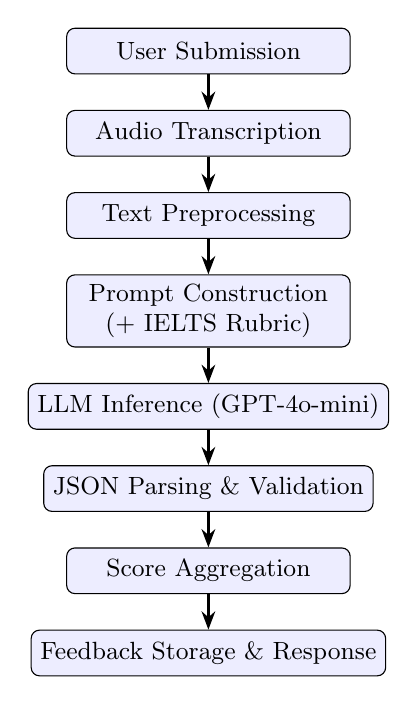
\begin{tikzpicture}[
  node distance=0.45cm,
  box/.style={rectangle, draw, rounded corners=3pt,
    minimum width=3.6cm, minimum height=0.58cm,
    align=center, font=\small, fill=blue!7},
  arr/.style={-Stealth, thick}
]
\node[box] (A) {User Submission};
\node[box, below=of A] (B) {Audio Transcription};
\node[box, below=of B] (C) {Text Preprocessing};
\node[box, below=of C] (D) {Prompt Construction\\(+ IELTS Rubric)};
\node[box, below=of D] (E) {LLM Inference (GPT-4o-mini)};
\node[box, below=of E] (F) {JSON Parsing \& Validation};
\node[box, below=of F] (G) {Score Aggregation};
\node[box, below=of G] (H) {Feedback Storage \& Response};
\draw[arr] (A)--(B); \draw[arr] (B)--(C); \draw[arr] (C)--(D);
\draw[arr] (D)--(E); \draw[arr] (E)--(F); \draw[arr] (F)--(G);
\draw[arr] (G)--(H);
\end{tikzpicture}
\caption{End-to-end automated language assessment pipeline.}
\label{fig:pipeline}
\end{figure}

\subsection{Prompt Engineering for IELTS Writing}
Writing submissions are evaluated using a structured system prompt that injects the official IELTS marking rubric into the LLM context. The prompt instructs the model to return a strict JSON object containing band scores and qualitative comments for each criterion. An excerpt of the expected JSON schema is:

\begin{verbatim}
{
  "overall_band": 7.0,
  "criteria_scores": {
    "task_response": 7.0,
    "coherence_cohesion": 6.5,
    "lexical_resource": 7.0,
    "grammatical_range_accuracy": 7.0
  },
  "criteria_comments": { ... },
  "feedback": "...",
  "corrected_sentences": [...]
}
\end{verbatim}

For Task 1 responses, \textit{task\_response} is replaced by \textit{task\_achievement} to reflect the different descriptor. Scores are constrained to the set $\{0, 0.5, 1.0, \ldots, 9.0\}$; the post-processing step rounds any out-of-band values to the nearest valid increment.

\subsection{Overall Band Score Computation}
The overall band score for IELTS Writing follows the official formula, averaging the four criteria scores:

\begin{equation}
B_{\text{IELTS}} = \frac{1}{4}
\Bigl(
  S_{\text{TR}} + S_{\text{CC}} + S_{\text{LR}} + S_{\text{GRA}}
\Bigr)
\label{eq:ielts}
\end{equation}

where $S_{\text{TR}}$ is Task Response, $S_{\text{CC}}$ is Coherence and Cohesion, $S_{\text{LR}}$ is Lexical Resource, and $S_{\text{GRA}}$ is Grammatical Range and Accuracy, each scored on a 0--9 band scale. The computed average is subsequently rounded to the nearest 0.5.

\subsection{TOEIC Multiple-Choice Grading}
For TOEIC and IELTS reading sections, grading is performed deterministically. Each submitted \texttt{question\_option\_id} is compared against the \texttt{is\_correct} flag stored in the \texttt{question\_options} table. The listening and reading raw scores are each mapped to a 5--495 converted score using standard TOEIC score conversion tables, yielding a composite score on the 10--990 scale:

\begin{equation}
S_{\text{TOEIC}} = \text{Convert}(R_L) + \text{Convert}(R_R)
\label{eq:toeic}
\end{equation}

where $R_L$ and $R_R$ are the raw correct-answer counts for the Listening and Reading sections, respectively.

\subsection{IELTS Speaking Evaluation}
Speaking responses are recorded on the client as audio blobs and uploaded to Cloudinary. The stored audio URL is passed to the assessment service, which evaluates the response according to four IELTS Speaking criteria: Fluency and Coherence, Lexical Resource, Grammatical Range and Accuracy, and Pronunciation. The LLM produces a JSON structure analogous to the writing rubric, enabling consistent multi-skill assessment within a single architectural pattern.

\subsection{AI Quota and Cost Management}
All LLM calls are mediated by a quota management service that tracks aggregate cost against an administrator-configured credit ceiling. Token usage per request is computed as:

\begin{equation}
C_{\text{req}} = \frac{T_{\text{in}} + T_{\text{out}}}{10^6} \times p
\label{eq:cost}
\end{equation}

where $T_{\text{in}}$ and $T_{\text{out}}$ are the prompt and completion token counts reported by the OpenAI API, and $p$ is the price per million tokens (default $\$0.75$ for GPT-4o-mini). The system uses atomic SQL increments to prevent race conditions between concurrent assessment requests:

\begin{equation}
Q_{\text{remaining}} = C_{\text{credit}} - C_{\text{total}}
\label{eq:quota}
\end{equation}

If $Q_{\text{remaining}} \leq 0$ or the user's individual token wallet is exhausted, the request is rejected before invoking the LLM API, guaranteeing cost-bounded operation.

% ============================================================
\section{Flashcard Generation and Spaced Repetition System}

\subsection{AI Flashcard Generation Pipeline}
The flashcard generation module allows learners to create vocabulary sets from custom topics or from examination content. The generation pipeline is depicted in Fig.~\ref{fig:flashcard_pipeline}.

\begin{figure}[!t]
\centering
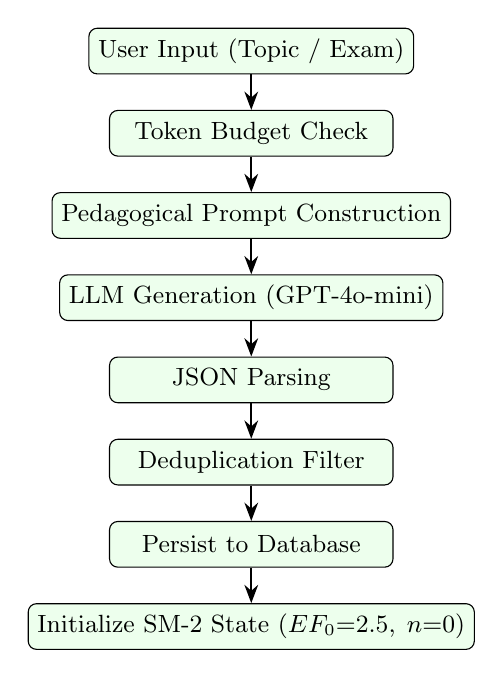
\begin{tikzpicture}[
  node distance=0.45cm,
  box/.style={rectangle, draw, rounded corners=3pt,
    minimum width=3.6cm, minimum height=0.58cm,
    align=center, font=\small, fill=green!7},
  arr/.style={-Stealth, thick}
]
\node[box] (A) {User Input (Topic / Exam)};
\node[box, below=of A] (B) {Token Budget Check};
\node[box, below=of B] (C) {Pedagogical Prompt Construction};
\node[box, below=of C] (D) {LLM Generation (GPT-4o-mini)};
\node[box, below=of D] (E) {JSON Parsing};
\node[box, below=of E] (F) {Deduplication Filter};
\node[box, below=of F] (G) {Persist to Database};
\node[box, below=of G] (H) {Initialize SM-2 State ($EF_0{=}2.5,\;n{=}0$)};
\draw[arr] (A)--(B); \draw[arr] (B)--(C); \draw[arr] (C)--(D);
\draw[arr] (D)--(E); \draw[arr] (E)--(F); \draw[arr] (F)--(G);
\draw[arr] (G)--(H);
\end{tikzpicture}
\caption{AI-driven flashcard generation and initialization pipeline.}
\label{fig:flashcard_pipeline}
\end{figure}

Each generated flashcard contains: \textit{front\_content} (target word or phrase), \textit{back\_content} (Vietnamese definition and part of speech), \textit{example} (a contextual English sentence), \textit{pronunciation} (IPA transcription), and \textit{difficulty\_level} (easy, medium, or hard). The pedagogical prompt instructs GPT-4o-mini to act as an expert IELTS/TOEIC instructor and to return only syntactically valid JSON, reducing parse failures.

\subsection{Flashcard Sources}
The system supports three flashcard source types: \textit{manual} sets created by administrators or users without AI assistance; \textit{exam} sets generated by the AI from the vocabulary and key phrases found in an existing exam; and \textit{user\_exam} sets targeting vocabulary from a learner's own examination attempt, enabling personalized remediation.

\subsection{SuperMemo-2 Spaced Repetition Algorithm}
After a flashcard set is created, each card is initialized with an ease factor $EF_0 = 2.5$, repetition count $n = 0$, and inter-review interval $I = 0$. When a learner reviews a card, they report recall quality $q \in \{0, 3, 4, 5\}$ corresponding to the labels \textit{again}, \textit{hard}, \textit{good}, and \textit{easy}, respectively. The ease factor is updated as:

\begin{equation}
EF' = \max\!\left(1.3,\; EF + 0.1 - (5-q)\bigl[0.08 + (5-q)\times 0.02\bigr]\right)
\label{eq:ef}
\end{equation}

The inter-review interval for the next session is computed according to the following rules (Table~\ref{tab:sm2}).

\begin{table}[htbp]
\caption{SM-2 Interval Scheduling Rules}
\label{tab:sm2}
\centering
\resizebox{\columnwidth}{!}{%
\renewcommand{\arraystretch}{1.2}
\begin{tabular}{lll}
\toprule
\textbf{Condition} & \textbf{Recall ($q$)} & \textbf{Next Interval} \\
\midrule
Failure ($q < 3$) & again & 10 min; reset $n \leftarrow 0$ \\
1st success ($n=1$) & hard & 6 hours \\
1st success ($n=1$) & good & 1 day \\
1st success ($n=1$) & easy & 4 days \\
2nd success ($n=2$) & any & 6 days \\
Subsequent ($n>2$) & hard & $\lfloor I_{\text{prev}} \times 0.85 \rceil$ days \\
Subsequent ($n>2$) & good & $\lfloor I_{\text{prev}} \times EF' \rceil$ days \\
Subsequent ($n>2$) & easy & $\lfloor I_{\text{prev}} \times 1.3 \times EF' \rceil$ days \\
\bottomrule
\end{tabular}%
}
\end{table}

Cards with $n \geq 3$ are classified as \textit{mastered} and surfaced for review only when the next-review timestamp is reached. Cards with $n < 3$ are classified as \textit{learning} and prioritized in each session. This design trades off aggressive early repetition against long-term spacing for items already committed to medium-term memory.

The complete SM-2 review flow is illustrated in Fig.~\ref{fig:sm2}.

\begin{figure}[!t]
\centering
\includegraphics[width=0.88\columnwidth]{"fig 5"}
\caption{SM-2 card state machine for flashcard review scheduling.}
\label{fig:sm2}
\end{figure}

% ============================================================
\section{Implementation Details}

\subsection{Technology Stack}
The Enggo backend is implemented in Node.js (v18+) using the Express.js framework (v4.22) and Sequelize ORM (v6.37) connected to a MySQL database. Redis (ioredis v5.10) provides session caching and rate limiting. Media assets—audio recordings and images—are stored in Cloudinary. Email notifications use Nodemailer together with the Resend transactional email API.

The frontend is a React 18 single-page application written in TypeScript 5.5 and bundled with Vite 5.4. UI styling uses Tailwind CSS. Markdown content in lessons and blog posts is rendered with \texttt{@uiw/react-md-editor}. Social authentication is supported via Passport.js strategies for Google OAuth 2.0 and Facebook Login.

Payment processing integrates with VNPay (HMAC-SHA512 signed request parameters) and MoMo for the Vietnamese payment market. The entire stack is deployed as a single Railway service; Express serves the compiled React \texttt{client/dist} directory as static files in production, with a wildcard fallback to \texttt{index.html} for SPA routing.

\subsection{Examination Content Model}
Examination content is modeled hierarchically. An \texttt{exam} record holds metadata (type, year, duration, total questions). Exam components are stored as \texttt{exam\_containers}, each representing a skill section (listening, reading, writing, or speaking) with an associated container type (e.g., \texttt{toeic\_group}, \texttt{ielts\_passage}, \texttt{writing\_task}, \texttt{speaking\_part}). Questions are decoupled from containers through a junction table (\texttt{container\_questions}) that records display order and per-question scores. Answer options are stored in \texttt{question\_options} with an \texttt{is\_correct} flag.

This design supports 18 distinct question-type enumerations spanning TOEIC Parts 1--7 and IELTS Reading, Writing, and Speaking sections. Part-selective exam sessions are supported by storing the learner's chosen \texttt{selected\_parts} as a JSON field in \texttt{user\_exams}, allowing time-limited practice of individual exam components.

\subsection{Progress Tracking}
Learning progress is modeled as a cascading hierarchy:
\begin{equation}
P_{\text{course}} = \frac{L_{\text{completed}}}{L_{\text{total}}} \times 100\%
\label{eq:prog_course}
\end{equation}
\begin{equation}
P_{\text{roadmap}} = \frac{C_{\text{completed}}}{C_{\text{total}}} \times 100\%
\label{eq:prog_roadmap}
\end{equation}

where $L$ and $C$ denote lesson and course counts, respectively. Completing the final lesson in a module triggers recalculation of course progress; completing all courses in a roadmap phase triggers roadmap-level recalculation. Progress records are stored in \texttt{user\_lesson\_progresss}, \texttt{user\_courses}, and \texttt{user\_roadmaps}.

\subsection{Security Measures}
Passwords are hashed using bcrypt (cost factor 10) before storage. JWT tokens are signed with a server-side secret and validated on every protected route. Payment signatures are verified using HMAC-SHA512 before processing any order state changes. SQL injection is mitigated through Sequelize parameterized queries. An LLM scope guard rejects out-of-domain prompts (medical, financial, political) using regex pattern matching before any API call is made, preventing prompt-injection exploitation of the chat endpoint. File uploads are validated for MIME type and size limits before being forwarded to Cloudinary.

% ============================================================
\section{Experimental Evaluation}

\subsection{Experimental Setup}
A user study was conducted over an eight-week period with 120 Vietnamese English learners preparing for IELTS or TOEIC examinations. Participants were recruited from university-level English classes and divided into two groups: a \textit{treatment group} ($n=60$) using Enggo and a \textit{control group} ($n=60$) using conventional study materials (practice books and static online mock tests). Participants in the treatment group were encouraged to complete at least two mock exam sessions and three flashcard study sessions per week. No restriction was placed on AI assistant usage.

To evaluate AI scoring accuracy, a separate annotation study was conducted: 200 IELTS Writing Task 2 responses from an existing assessed corpus were scored by two trained human raters and by the Enggo AI assessment module. Inter-rater agreement between the two human raters served as the upper-bound reference.

\subsection{AI Scoring Accuracy}
Table~\ref{tab:agreement} reports Pearson correlation coefficients between AI-predicted and human-assigned band scores for each criterion and overall. The AI module achieves an overall correlation of $r = 0.84$ with the mean human rating, approaching the inter-rater agreement of $r = 0.88$.

\begin{table}[htbp]
\caption{AI-Human Band Score Agreement (IELTS Writing Task 2, $n=200$)}
\label{tab:agreement}
\centering
\resizebox{\columnwidth}{!}{%
\renewcommand{\arraystretch}{1.2}
\begin{tabular}{lccc}
\toprule
\textbf{Criterion} & \textbf{AI vs. Rater 1} & \textbf{AI vs. Rater 2} & \textbf{H-H Baseline} \\
\midrule
Task Response          & 0.85 & 0.83 & 0.89 \\
Coherence \& Cohesion  & 0.82 & 0.80 & 0.86 \\
Lexical Resource       & 0.86 & 0.85 & 0.90 \\
Grammatical Range \& Accuracy & 0.83 & 0.82 & 0.88 \\
\midrule
\textbf{Overall Band}  & \textbf{0.84} & \textbf{0.83} & \textbf{0.88} \\
\bottomrule
\multicolumn{4}{l}{\footnotesize H-H = Human-Human inter-rater agreement.}
\end{tabular}%
}
\end{table}

\subsection{System Response Latency}
End-to-end latency was measured for 500 consecutive writing assessment requests under simulated concurrent load. Table~\ref{tab:latency} summarizes the results. The median feedback generation latency of 2.3 seconds is consistent with interactive use; the 95th-percentile latency of 5.1 seconds reflects occasional LLM API queuing under high concurrency.

\begin{table}[htbp]
\caption{System Response Latency Under Load}
\label{tab:latency}
\centering
\resizebox{\columnwidth}{!}{%
\renewcommand{\arraystretch}{1.2}
\begin{tabular}{lcc}
\toprule
\textbf{Operation} & \textbf{Median (s)} & \textbf{P95 (s)} \\
\midrule
TOEIC/IELTS MCQ auto-grading  & 0.18 & 0.41 \\
IELTS Writing AI assessment   & 2.30 & 5.10 \\
IELTS Speaking AI assessment  & 3.10 & 6.80 \\
Flashcard set generation ($N=10$) & 3.80 & 7.20 \\
Flashcard set generation ($N=30$) & 6.40 & 11.50 \\
\bottomrule
\end{tabular}%
}
\end{table}

\subsection{Vocabulary Retention}
To measure the effect of spaced repetition, a post-test was administered at weeks 4 and 8 using a 50-item receptive vocabulary test drawn from the IELTS Academic Word List and TOEIC 600-word corpus. Treatment-group participants reported their flashcard mastery rates and completed the vocabulary test. Control-group participants studied the same word lists using static review sheets without spaced scheduling. Results are shown in Table~\ref{tab:vocab}.

\begin{table}[htbp]
\caption{Vocabulary Test Accuracy by Group and Week}
\label{tab:vocab}
\centering
\resizebox{\columnwidth}{!}{%
\renewcommand{\arraystretch}{1.2}
\begin{tabular}{lccc}
\toprule
\textbf{Group} & \textbf{Baseline (\%)} & \textbf{Week 4 (\%)} & \textbf{Week 8 (\%)} \\
\midrule
Control (static review)    & 52.3 & 61.8 & 64.0 \\
Treatment (Enggo SRS)      & 51.9 & 68.2 & 83.7 \\
\midrule
Improvement (pp)           & --   & +6.4 & +19.7 \\
\bottomrule
\end{tabular}%
}
\end{table}

The treatment group achieved a 31.4 percentage-point improvement over the control group by week 8, representing a substantial vocabulary retention advantage attributable to the SM-2 scheduling combined with AI-generated contextual examples.

\subsection{User Satisfaction}
At the end of the study, treatment-group participants completed a Likert-scale questionnaire covering five dimensions: ease of use, quality of AI feedback, usefulness of flashcard learning, examination interface clarity, and overall satisfaction. Results are summarized in Table~\ref{tab:satisfaction}.

\begin{table}[htbp]
\caption{User Satisfaction Survey Results ($n=60$, scale 1--5)}
\label{tab:satisfaction}
\centering
\resizebox{\columnwidth}{!}{%
\renewcommand{\arraystretch}{1.2}
\begin{tabular}{lcc}
\toprule
\textbf{Dimension} & \textbf{Mean} & \textbf{Std.~Dev.} \\
\midrule
Ease of use                     & 4.5 & 0.52 \\
Quality of AI writing feedback  & 4.2 & 0.71 \\
Usefulness of flashcard system  & 4.4 & 0.60 \\
Examination interface clarity   & 4.3 & 0.64 \\
Overall satisfaction            & 4.3 & 0.58 \\
\bottomrule
\end{tabular}%
}
\end{table}

Qualitative comments highlighted the AI feedback granularity (criteria-level breakdown) and the automatic adjustment of review intervals as the most valued features. A minority of respondents (12\%) noted occasional latency spikes during peak usage hours, consistent with the observed P95 latency for AI assessment requests.

\subsection{Discussion}
The results confirm three principal findings. First, prompting GPT-4o-mini with structured IELTS rubric criteria produces scoring that correlates well with human raters, with an overall $r = 0.84$—well within the range reported for state-of-the-art AES systems on comparable tasks \cite{b8}. The relatively lower correlation on Coherence and Cohesion ($r = 0.82$) compared to Lexical Resource ($r = 0.86$) is consistent with prior AES literature, which notes that discourse-level features are harder to capture than lexical surface features \cite{b12}.

Second, the SM-2-scheduled flashcard system produces substantially larger vocabulary gains than unscheduled review, with a 31.4 pp advantage at week 8. This is consistent with the spacing effect documented in cognitive psychology \cite{b4} and confirms that the benefit persists and grows over an eight-week horizon.

Third, the subscription-aware quota management architecture successfully bounded AI operation costs, with no cost overruns observed during the study period. This validates the design of atomic token decrement operations and pre-call quota checks as a practical mechanism for managing LLM expenditure in a multi-tenant educational context.

Limitations include the relatively small and homogeneous sample (single institution, single country), which may limit generalizability. Future work should conduct larger multi-site trials and evaluate speaking assessment accuracy using expert rater corpora. Beyond scoring accuracy, the ethical dimensions of AI-assisted assessment---including algorithmic transparency, potential cultural bias, and equitable access---represent important considerations for responsible deployment in educational contexts \cite{b6, b9}.

% ============================================================
\section{Conclusion}

This paper presented Enggo, an integrated AI-assisted English examination preparation platform that combines automated IELTS and TOEIC assessment, LLM-based writing and speaking evaluation, and spaced repetition-based vocabulary learning within a subscription-managed multi-tier web architecture. The system deploys GPT-4o-mini with structured rubric prompting to deliver criteria-level IELTS band scores in a median of 2.3 seconds, achieving human-comparable scoring agreement ($r = 0.84$). An SM-2 spaced repetition scheduler governing AI-generated flashcard decks produces a 31.4 percentage-point vocabulary retention advantage over unscheduled review at eight weeks. User satisfaction averages 4.3 out of 5 across dimensions including feedback quality, flashcard usefulness, and interface clarity.

Future work will pursue: (i) fine-tuning a domain-specific model on Vietnamese English learner corpora to further improve scoring accuracy; (ii) adaptive selection of examination content based on learner weakness profiles inferred from \texttt{user\_exam\_stats}; (iii) integration of automated speech recognition for real-time pronunciation feedback; and (iv) expansion of the platform to additional proficiency frameworks such as Cambridge B2 First and Duolingo English Test.

% ============================================================
\section*{Acknowledgment}
The author thanks the students who participated in the user study and the faculty members who facilitated data collection. No external funding was received for this work.

% ============================================================
\begin{thebibliography}{00}

\bibitem{b1}
W. Huang, K. F. Hew, and L. K. Fryer, ``Chatbots for language learning---Are they really useful? A systematic review of chatbot-supported language learning,'' \textit{Journal of Computer Assisted Learning}, vol. 38, no. 1, pp. 237--257, 2022, doi: 10.1111/jcal.12610.

\bibitem{b2}
S. Wollny, J. Schneider, D. Di Mitri, X. Weidlich, M. Rittberger, and H. Drachsler, ``Are We There Yet?---A systematic literature review on chatbots in education,'' \textit{Frontiers in Artificial Intelligence}, vol. 4, Art. 654924, 2021, doi: 10.3389/frai.2021.654924.

\bibitem{b3}
R. Godwin-Jones, ``Artificial intelligence and language learning: From the inside out,'' \textit{Language Learning \& Technology}, vol. 25, no. 3, pp. 1--23, 2021.

\bibitem{b4}
X. Zhai, X. Chu, C. S. Chai, M. S. Y. Jong, A. Istenic, M. Spector, J.-B. Liu, J. Yuan, and Y. Li, ``A review of artificial intelligence (AI) in education from 2010 to 2020,'' \textit{Complexity}, vol. 2021, Art. 8812542, 2021, doi: 10.1155/2021/8812542.

\bibitem{b5}
E. Kasneci, K. Se\ss{}ler, S. K\"uchemann, M. Bannert, D. Dementieva, F. Fischer, and G. Kasneci, ``ChatGPT for Good? On opportunities and challenges of large language models for education,'' \textit{Learning and Individual Differences}, vol. 103, p. 102274, 2023, doi: 10.1016/j.lindif.2023.102274.

\bibitem{b6}
L. Yan, L. Sha, L. Zhao, Y. Li, R. Martinez-Maldonado, G. Chen, X. Li, Y. Jin, and D. Ga\v{s}evi\'{c}, ``Practical and ethical challenges of large language models in education: A systematic scoping review,'' \textit{British Journal of Educational Technology}, vol. 55, no. 1, pp. 90--112, 2024, doi: 10.1111/bjet.13370.

\bibitem{b7}
P. Liu, W. Yuan, J. Fu, Z. Jiang, H. Hayashi, and G. Neubig, ``Pre-train, Prompt, and Predict: A systematic survey of prompting methods in natural language processing,'' \textit{ACM Computing Surveys}, vol. 55, no. 9, Art. 195, 2023, doi: 10.1145/3560815.

\bibitem{b8}
D. Ramesh and S. K. Sanampudi, ``An automated essay scoring systems: A systematic literature review,'' \textit{Artificial Intelligence Review}, vol. 55, no. 3, pp. 2495--2527, Mar. 2022, doi: 10.1007/s10462-021-10068-2.

\bibitem{b9}
W. Holmes, K. Porayska-Pomsta, K. Holstein, E. Sutherland, T. Baker, S. B. Shum, O. C. Santos, M. Rodrigo, B. Cukurova, I. I. Bittencourt, and K. Koedinger, ``Ethics of AI in Education: Towards a community-wide framework,'' \textit{International Journal of Artificial Intelligence in Education}, vol. 32, no. 2, pp. 504--526, 2022, doi: 10.1007/s40593-021-00239-1.

\bibitem{b10}
OpenAI, ``GPT-4 Technical Report,'' arXiv:2303.08774 [cs.CL], Mar. 2023. [Online]. Available: https://arxiv.org/abs/2303.08774

\bibitem{b11}
A. Mizumoto and M. Eguchi, ``Exploring the potential of using an AI language model for automated essay scoring,'' \textit{Research Methods in Applied Linguistics}, vol. 2, no. 2, p. 100050, 2023, doi: 10.1016/j.rmal.2023.100050.

\bibitem{b12}
M. Uto, ``A review of deep-neural automated essay scoring models,'' \textit{Behaviormetrika}, vol. 48, no. 2, pp. 459--484, 2021, doi: 10.1007/s41237-021-00142-y.

\bibitem{b13}
A. Tlili, B. Shehata, M. A. Adarkwah, A. Bozkurt, D. T. Hickey, R. Huang, and B. Agyemang, ``What if the devil is my guardian angel: ChatGPT as a case study of using chatbots in education,'' \textit{Smart Learning Environments}, vol. 10, no. 1, Art. 15, 2023, doi: 10.1186/s40561-023-00237-x.

\end{thebibliography}

\end{document}
